% !TeX program = lualatex


\documentclass[aspectratio=169,xcolor={dvipsnames}
%,notes=only
%,notes
%,show notes on second screen=right
,handout
]{beamer}
\usetheme[background=light, numbering=fraction]{metropolis}
\usepackage{appendixnumberbeamer}
\usepackage{pgfpages}

%\usepackage[T1]{fontenc}

\usepackage{bm}
\usepackage{mathtools}

\usepackage[labelfont=bf,textfont={it}]{caption}
\usepackage{subcaption}
\captionsetup[figure]{justification=centering}
\captionsetup[subfigure]{justification=centering}

\usepackage{tikz}
\usetikzlibrary{arrows.meta, calc, fit, positioning}

%\usepackage{fontspec}
%\setsansfont{Fira Sans Mono}

\usepackage{etoolbox}
\usepackage[binary-units]{siunitx}
\robustify\bfseries
\sisetup{detect-all, range-phrase=--, range-units=single}

\usepackage[UKenglish]{babel}
\usepackage{csquotes}

\usepackage{amssymb}

\usepackage{lipsum}
%\usepackage[basic]{complexity}
\usepackage[super,negative]{nth}

\usepackage{booktabs}

%bib
\usepackage[maxnames=3,maxbibnames=99,mincrossrefs=5,sortcites
%,backend=bibtex
,style=authortitle
]{biblatex}
\addbibresource{../paper/papers-off.bib}
\addbibresource{../paper/confs-off.bib}

\newcommand{\acval}[3]{\ensuremath{\operatorname{\hat{q}}(#1, #2, #3)}}
\newcommand{\wvec}[1]{\ensuremath{\bm{w}_{#1}}}

\makeatletter
\DeclareRobustCommand{\rvdots}{%
	\vbox{
		\baselineskip4\p@\lineskiplimit\z@
		\kern-\p@
		\hbox{.}\hbox{.}\hbox{.}
}}
\makeatother

% official colours
\definecolor{uofguniversityblue}{rgb}{0, 0.219608, 0.396078}

\definecolor{uofgheather}{rgb}{0.356863, 0.32549, 0.490196}
\definecolor{uofgaquamarine}{rgb}{0.603922, 0.72549, 0.678431}
\definecolor{uofgslate}{rgb}{0.309804, 0.34902, 0.380392}
\definecolor{uofgrose}{rgb}{0.823529, 0.470588, 0.709804}
\definecolor{uofgmocha}{rgb}{0.709804, 0.564706, 0.47451}

\definecolor{uofglawn}{rgb}{0.517647, 0.741176, 0}
\definecolor{uofgcobalt}{rgb}{0, 0.615686, 0.92549}
\definecolor{uofgturquoise}{rgb}{0, 0.709804, 0.819608}
\definecolor{uofgsunshine}{rgb}{1.0, 0.862745, 0.211765}
\definecolor{uofgpumpkin}{rgb}{1.0, 0.72549, 0.282353}
\definecolor{uofgthistle}{rgb}{0.584314, 0.070588, 0.447059}
\definecolor{uofgpillarbox}{rgb}{0.701961, 0.047059, 0}
\definecolor{uofglavendar}{rgb}{0.356863, 0.301961, 0.580392}

\definecolor{uofgsandstone}{rgb}{0.321569, 0.278431, 0.231373}
\definecolor{uofgforest}{rgb}{0, 0.317647, 0.2}
\definecolor{uofgburgundy}{rgb}{0.490196, 0.133333, 0.223529}
\definecolor{uofgrust}{rgb}{0.603922, 0.227451, 0.023529}

\definecolor{inferno0}{rgb}{0.001462 0.000466 0.013866}
\definecolor{inferno64}{rgb}{0.341500 0.062325 0.429425}
\definecolor{inferno128}{rgb}{0.735683 0.215906 0.330245}
\definecolor{inferno192}{rgb}{0.978422 0.557937 0.034931}
\definecolor{inferno255}{rgb}{0.988362 0.998364 0.644924}

%picky abt et al.
\usepackage{xpatch}

\makeatletter\let\expandableinput\@@input\makeatother

\xpatchbibmacro{name:andothers}{%
	\bibstring{andothers}%
}{%
	\bibstring[\emph]{andothers}%
}{}{}

%opening!

\usepackage{cleveref}
\newcommand{\crefrangeconjunction}{--}

\usepackage{fontawesome}

\addtobeamertemplate{footnote}{\vspace{-6pt}\advance\hsize-0.5cm}{\vspace{6pt}}
\makeatletter
% Alternative A: footnote rule
\renewcommand*{\footnoterule}{\kern -3pt \hrule \@width 2in \kern 8.6pt}
% Alternative B: no footnote rule
% \renewcommand*{\footnoterule}{\kern 6pt}
\makeatother

\usepackage[export]{adjustbox}
\usetikzlibrary{arrows.meta, calc, fit, positioning, shapes.misc}

\newcommand{\approach}{On Path Learning}
\newcommand{\approachshort}{OPaL}
\newcommand{\Coopfw}{\emph{CoOp}}
\newcommand{\coopfw}{\Coopfw}
\newcommand{\Indfw}{\emph{Ind}}
\newcommand{\indfw}{\Indfw}
\newcommand{\inring}{\textsc{In}}
\newcommand{\outring}{\textsc{Out}}

\makeatletter\let\expandableinput\@@input\makeatother
\newcommand{\cmark}{\ding{51}}%
\newcommand{\xmark}{\ding{55}}%

%-------------------------------------%
%-------------------------------------%

\title{Revisiting the Classics: Online RL in the Programmable Dataplane}
\author{\vspace{-1em}\textbf{Kyle A. Simpson}, Dimitrios P. Pezaros\\
	\faEnvelopeO{} \href{mailto:k.simpson.1@research.gla.ac.uk}{\nolinkurl{k.simpson.1@research.gla.ac.uk}}\\
	\vspace{1em}\small{\faGithub{} \href{https://github.com/felixmcfelix}{FelixMcFelix} \hspace{0.5em} \faGlobe{} \url{https://mcfelix.me}}}
\institute{University of Glasgow}
\date{\nth{4} June, 2021}

\begin{document}
% title fun, including Org logos....
\begin{frame}
	\maketitle
	\begin{tikzpicture}[overlay, remember picture]
%		\node[above right=0.8cm and 0.9cm of current page.south west] (esnet-logo) {\includegraphics[width=2.75cm]{netlab-trim}};
%		\node[right=1cm of esnet-logo] {\adjincludegraphics[height=2cm,trim={0 {.4\height} 0 {.05\height}},clip]{uofg}};
		\node[above right=-0.1cm and 0.8cm of current page.south west] (uofg-logo) {\adjincludegraphics[height=2cm,trim={0 {.4\height} 0 {.05\height}},clip]{uofg}};
		\node[right=0.5cm of uofg-logo] {\includegraphics[width=2.75cm]{netlab-trim}};
	\end{tikzpicture}
\end{frame}

\begin{frame}{Data-driven networking: RL in networks}
	\alert{Data-driven networking}: Automate control, optimisation, configuration of the network.
	\begin{itemize}
		\item Flow performance optimisation.
		\item Resource allocation.
		\item Adaptive response to load, intrusions, etc.
		\item Feedback loop-like.
	\end{itemize}
\end{frame}

\begin{frame}{Why programmable data-planes?}
	\begin{columns}
		\begin{column}{0.6\linewidth}
			\begin{figure}
				\resizebox{\linewidth}{!}{
					\begin{tikzpicture}
						\node (iLabel) {Theory};
						
						\node (iDiag) at ($(0, -1.3) + (iLabel)$) {
							\resizebox{2cm}{!}{\begin{tikzpicture}
									\node[circle, draw] (state) {$S$};
									\node[circle, draw] (state') at ($(state) + (0, -2)$) {$S'$};
									
									\node (agent) at ($(2, 0) + (state)$) {Agent};
									\node[below of=agent] (action) {Action $A$};
									
									\node[right of=state'] {$+ R$};
									
									\draw[->] (state) -- (state') node[midway, right] {$A$};
									
									\draw[dotted, ->, bend left = 30] (state) -- (agent);
									\draw[->] (agent) -- (action);
									\draw[dotted, ->] (action) -- (state);
						\end{tikzpicture}}};
						
						\node (rLabel) at ($(3, 0) + (iLabel)$) {Reality};
						
						\node (rDiag) at ($(0, -1.5) + (rLabel)$) {
							\resizebox{2cm}{!}{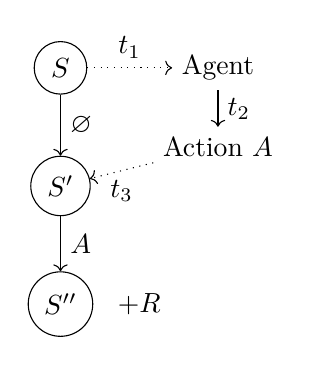
\begin{tikzpicture}
									\node[circle, draw] (state) {$S$};
									\node[circle, draw] (state') at ($(state) + (0, -1.5)$) {$S'$};
									\node[circle, draw] (state'') at ($(state') + (0, -1.5)$) {$S''$};
									
									\node (agent) at ($(2, 0) + (state)$) {Agent};
									\node[below of=agent] (action) {Action $A$};
									
									\node[right of=state''] {$+ R$};
									
									\draw[->] (state) -- (state') node[midway, right] {$\varnothing$};
									\draw[->] (state') -- (state'') node[midway, right] {$A$};
									
									\draw[dotted, ->, bend left = 30] (state) -- (agent) node[midway, above] {$t_1$};
									\draw[->] (agent) -- (action) node[midway, right] {$t_2$};
									\draw[dotted, ->] (action) -- (state') node[midway, below] {$t_3$};
						\end{tikzpicture}}};
					\end{tikzpicture}
				}
				\caption{Asynchronous RL delays and state slippage (policy updates omitted).}
			\end{figure}
		\end{column}
		\begin{column}{0.4\linewidth}
			\begin{itemize}
				\item In data-driven, want to \alert{minimise time to act}.
				\item RL assumes that action \& policy update are zero-cost.
				\vspace{-1em}
				\begin{itemize}
					\item Not so in real deployments!
					\item State drift, etc.
				\end{itemize}
				\item Controller contact time, serialisation, ...
				\item In other ML, often need line rate inference.
				\item Programmable network hardware fills this niche.
			\end{itemize}
		\end{column}
	\end{columns}
\end{frame}

\begin{frame}{Recent Programmable Trends in Data-Driven Networks}
	\begin{columns}
		\begin{column}{0.6\linewidth}
			\begin{itemize}
				\item ML acceleration, line-rate packet classification.
				\item How? Train model off-NIC, convert to \alert{binary neural network}\footnotemark, or \alert{decision tree}\footnotemark.
				\item Limits? No online training, cost of backprop algo (expensive!), vast data needs.
				\item \alert{What if we need online learning?}
			\end{itemize}
		\end{column}
		\begin{column}{0.4\linewidth}
			\centering
			\resizebox{0.6\linewidth}{!}{
				\includegraphics{images/smartnic.png}
			}
		
			\resizebox{0.5\linewidth}{!}{
				\includegraphics{images/nn}
			}
		\end{column}
	\end{columns}
\setcounter{footnote}{1}
\footcitetext{DBLP:journals/corr/abs-2009-02353}
\setcounter{footnote}{2}
\footcitetext{DBLP:conf/hotnets/XiongZ19}
\end{frame}

\begin{frame}{Timing: Why not offload to the controller?}
	\begin{columns}
		\begin{column}{0.5\linewidth}
			For SmartNICs, the attached host \emph{is the (closest) controller}.
			
			\begin{itemize}
				\item PCIe access times $\mathcal{O}(\si{\micro\second})$\footnotemark
				\item Crossing VMs/vNFS has $\sim$\SI{10}{$\times$} higher cost\footnotemark
				\item MATs recompiled $\mathcal{O}(\si{\second})$. Many rules $\implies$ batching.
%				\item Thrift serde time $\mathcal{O}(\si{\milli\second})$.
			\end{itemize}
			
			%	?? https://github.com/rpclib/benchmarks/blob/master/plots/get_blob_real_log.svg
			
			\alert{Meanwhile core-to-core on NFP around \SI{140}{\nano\second} @ \SI{1.2}{\giga\hertz}.}
		\end{column}
		\begin{column}{0.5\linewidth}
			\begin{figure}
				\includegraphics[width=0.9\linewidth]{../plots/build/rte-timer/rte-times-logx}
				\caption{Netronome rule installation cost \\(1 table, \numrange{1}{65536} rules).}
			\end{figure}
		\end{column}
	\end{columns}
	\setcounter{footnote}{3}
	\footcitetext{DBLP:conf/sigcomm/NeugebauerAZAL018}
	\setcounter{footnote}{4}
	\footcitetext{DBLP:journals/cm/CzivaP17}
\end{frame}

\begin{frame}{How do we bring online, in-NIC RL?}
	\begin{columns}
		\begin{column}{0.6\linewidth}
			\begin{figure}
				\includegraphics[width=\linewidth]{../paper/figures/arch-with-p4}
			\end{figure}
		\end{column}
		\begin{column}{0.4\linewidth}
			\begin{itemize}
				\item Classical RL built on tile-coding---\alert{online}.
				\item \alert{Fixed-point arithmetic}.
				\item Async wrt. datapath.
				\item Dynamic selection of last reward, trace info.
				\item \alert{Runtime configurable} (policy, size, application) from data/control-plane. \alert{Task independent.}
			\end{itemize}
		\end{column}
	\end{columns}
\end{frame}

\section{Background and Design}

\begin{frame}{Single-step (classical) RL---Sarsa}
	A simple explanation:\pause
	
	\begin{subequations}
		\begin{gather}
			\delta_t = \overbrace{R_{t+1} + \gamma \acval{S_{t+1}}{A_{t+1}}{\wvec{t}}}^{\mathclap{\substack{\text{New target value:}\\ \text{Reward} + \text{some of the next action's value}}}} - \underbrace{\acval{S_t}{A_t}{\wvec{t}}}_{\mathclap{\text{Current value estimate}}},\\\pause
			\bm{w}_{t+1} = \bm{w}_{t} + \overbrace{\alpha \delta_t}^{\mathclap{\text{Move a little bit of } \delta_t \text{ along...}}} \underbrace{\nabla{\acval{S_t}{A_t}{\wvec{t}}}}_{\mathclap{\text{...the policy's gradient}}},\pause
		\end{gather}%
	\end{subequations}

	Design implications?
\end{frame}

\begin{frame}{Tile Coding}
\centering
\resizebox{0.7\linewidth}{!}{
	\begin{tikzpicture}
		\node at (0.35,0.4){$s = \begin{pmatrix}
				0.7 \\
				0.3
			\end{pmatrix}$};
		\node at (0,-1.1) {$\bm{x}(s,\cdot) = \begin{Bmatrix}
				T_{1,9}, \\
				T_{2,5}, \\
				T_{\mathit{bias}}
			\end{Bmatrix}$};
		
		\node at (2.5,-0.5) {
			\begin{tikzpicture}
				\draw[step=0.5cm,color=uofgcobalt,opacity=0.7,shift={(0,0)},label=above:{Tiling 0}] (-0.5,-0.5) grid (1,1);
				\fill[uofgcobalt,opacity=0.5] (0.5,-0.5) rectangle (1,0);
				\node[color=uofgcobalt] at (0,1.2) {\footnotesize Tiling 1};
				
				\draw[step=0.5cm,color=uofgpumpkin,opacity=0.9,shift={(0.25,-0.25)},label=above:{Tiling 1}] (-0.5,-0.5) grid (1,1);
				\fill[uofgpumpkin,opacity=0.5,shift={(0.25,-0.25)}] (0,0) rectangle (0.5,0.5);
				\node[color=uofgpumpkin!50!uofgrust] at (0.25,-0.95) {\footnotesize Tiling 2};
				
				\node[circle, black, draw,
				fill, radius=0.5pt, inner sep=0pt,minimum size=1.5pt, label=above:{$s$}] at (0.625,-0.125) {};
				%			\filldraw (0.625,-0.125) circle[radius=1.5pt,label=above:{$s$}];
				
				\draw[->] (-0.25,-0.5)--(-0.25,0.85);
				\draw[->] (-0.25,-0.5)--(1.1,-0.5);
				
				\node at (1,-0.7) {\footnotesize 1};
				\node at (-0.4,0.75) {\footnotesize 1};
				\node at (-0.35,-0.6) {\footnotesize 0};
			\end{tikzpicture}
		};
		
	\end{tikzpicture}
}
\end{frame}

\begin{frame}{Tile Coding (ii)}
	\begin{columns}
		\begin{column}{0.6\linewidth}
			\centering
			\resizebox{0.8\linewidth}{!}{
				\begin{tikzpicture}
					\node at (0.35,0.4){$s = \begin{pmatrix}
							0.7 \\
							0.3
						\end{pmatrix}$};
					\node at (0,-1.1) {$\bm{x}(s,\cdot) = \begin{Bmatrix}
							T_{1,9}, \\
							T_{2,5}, \\
							T_{\mathit{bias}}
						\end{Bmatrix}$};
					
					\node at (2.5,-0.5) {
						\begin{tikzpicture}
							\draw[step=0.5cm,color=uofgcobalt,opacity=0.7,shift={(0,0)},label=above:{Tiling 0}] (-0.5,-0.5) grid (1,1);
							\fill[uofgcobalt,opacity=0.5] (0.5,-0.5) rectangle (1,0);
							\node[color=uofgcobalt] at (0,1.2) {\footnotesize Tiling 1};
							
							\draw[step=0.5cm,color=uofgpumpkin,opacity=0.9,shift={(0.25,-0.25)},label=above:{Tiling 1}] (-0.5,-0.5) grid (1,1);
							\fill[uofgpumpkin,opacity=0.5,shift={(0.25,-0.25)}] (0,0) rectangle (0.5,0.5);
							\node[color=uofgpumpkin!50!uofgrust] at (0.25,-0.95) {\footnotesize Tiling 2};
							
							\node[circle, black, draw,
							fill, radius=0.5pt, inner sep=0pt,minimum size=1.5pt, label=above:{$s$}] at (0.625,-0.125) {};
							%			\filldraw (0.625,-0.125) circle[radius=1.5pt,label=above:{$s$}];
							
							\draw[->] (-0.25,-0.5)--(-0.25,0.85);
							\draw[->] (-0.25,-0.5)--(1.1,-0.5);
							
							\node at (1,-0.7) {\footnotesize 1};
							\node at (-0.4,0.75) {\footnotesize 1};
							\node at (-0.35,-0.6) {\footnotesize 0};
						\end{tikzpicture}
					};
					
				\end{tikzpicture}
			}
		\end{column}
		\begin{column}{0.4\linewidth}
			\begin{itemize}[<+->]
				\item Operations? $+, -, \times, \div$
				\begin{itemize}[<+->]
					\item PoT tile width? $\div$ replaced w/ shift.
				\end{itemize}
				\item Tiling set: identical dimensions, different shifts
				\item Gradient for RL?
				\begin{itemize}[<+->]
					\item List of hit tiles.
				\end{itemize}
				\item Can be more complex...
			\end{itemize}
		\end{column}
	\end{columns}
\end{frame}

\begin{frame}{Tile Coding: Parallelism}
	\centering
	\resizebox{0.7\linewidth}{!}{
		\begin{tikzpicture}
			\node at (0,0) {
				\begin{tikzpicture}
					\draw[step=0.5cm,color=uofgcobalt,opacity=0.7,shift={(0,0)},label=above:{Tiling 0}] (-0.5,-0.5) grid (1,1);
					\fill[uofgcobalt,opacity=0.5] (0.5,-0.5) rectangle (1,0);
					\node[color=uofgcobalt] (t1g) at (0,1.2) {\footnotesize Tiling 1};
					
					\draw[step=0.5cm,color=uofgpumpkin,opacity=0.9,shift={(0.25,-0.25)},label=above:{Tiling 1}] (-0.5,-0.5) grid (1,1);
					\fill[uofgpumpkin,opacity=0.5,shift={(0.25,-0.25)}] (0,0) rectangle (0.5,0.5);
					\node[color=uofgpumpkin!50!uofgrust] (t2g) at (0.25,-0.95) {\footnotesize Tiling 2};
					
					\node[circle, black, draw,
					fill, radius=0.5pt, inner sep=0pt,minimum size=1.5pt, label=above:{$s$}] at (0.625,-0.125) {};
					%			\filldraw (0.625,-0.125) circle[radius=1.5pt,label=above:{$s$}];
					
					\draw[->] (-0.25,-0.5)--(-0.25,0.85);
					\draw[->] (-0.25,-0.5)--(1.1,-0.5);
					
					\node at (1,-0.7) {\footnotesize 1};
					\node at (-0.4,0.75) {\footnotesize 1};
					\node at (-0.35,-0.6) {\footnotesize 0};
				\end{tikzpicture}
			};
		
		\node (policy-head) at (2.5,1.2) {Policy};
		\draw[color=uofgcobalt,opacity=0.7] (2,0) rectangle ++(2,1) node[pos=.5] (t1p) {Tiling 1};
		\fill[uofgcobalt,opacity=0.25] (3.33,0) rectangle ++(0.67,0.33);
		
		\draw[color=uofgpumpkin,opacity=0.9] (2,-1) rectangle ++(2,1) node[pos=.5] (t2p) {Tiling 2};
		\fill[uofgpumpkin,opacity=0.25] (2.67,-0.67) rectangle ++(0.67,0.33);
		
		\draw (2,-2) rectangle ++(2,1) node[pos=.5] {$\cdots$};
		
		\draw [->,color=uofgcobalt, bend left] (t1g) to (t1p.west);
		\draw [->,color=uofgpumpkin, bend right] (t2g) to (t2p.west);
			
		\end{tikzpicture}
	}
\end{frame}

\begin{frame}{Tile Coding: Parallelism (ii)}
	\centering
	\resizebox{0.6\linewidth}{!}{
		\begin{tikzpicture}
			\node at (0,0) {
				\begin{tikzpicture}
					\draw[step=0.5cm,color=uofgcobalt,opacity=0.7,shift={(0,0)},label=above:{Tiling 0}] (-0.5,-0.5) grid (1,1);
					\fill[uofgcobalt,opacity=0.5] (0.5,-0.5) rectangle (1,0);
					\node[color=uofgcobalt] (t1g) at (0,1.2) {\footnotesize Tiling 1};
					
					\draw[step=0.5cm,color=uofgpumpkin,opacity=0.9,shift={(0.25,-0.25)},label=above:{Tiling 1}] (-0.5,-0.5) grid (1,1);
					\fill[uofgpumpkin,opacity=0.5,shift={(0.25,-0.25)}] (0,0) rectangle (0.5,0.5);
					\node[color=uofgpumpkin!50!uofgrust] (t2g) at (0.25,-0.95) {\footnotesize Tiling 2};
					
					\node[circle, black, draw,
					fill, radius=0.5pt, inner sep=0pt,minimum size=1.5pt, label=above:{$s$}] at (0.625,-0.125) {};
					%			\filldraw (0.625,-0.125) circle[radius=1.5pt,label=above:{$s$}];
					
					\draw[->] (-0.25,-0.5)--(-0.25,0.85);
					\draw[->] (-0.25,-0.5)--(1.1,-0.5);
					
					\node at (1,-0.7) {\footnotesize 1};
					\node at (-0.4,0.75) {\footnotesize 1};
					\node at (-0.35,-0.6) {\footnotesize 0};
				\end{tikzpicture}
			};
			
			\node (policy-head) at (2.5,1.2) {Policy};
			\draw[color=uofgcobalt,opacity=0.7] (2,0) rectangle ++(2,1) node[pos=.5] (t1p) {Tiling 1};
			\fill[uofgcobalt,opacity=0.25] (3.33,0) rectangle ++(0.67,0.33);
			
			\draw[color=uofgpumpkin,opacity=0.9] (2,-1) rectangle ++(2,1) node[pos=.5] (t2p) {Tiling 2};
			\fill[uofgpumpkin,opacity=0.25] (2.67,-0.67) rectangle ++(0.67,0.33);
			
			\draw (2,-2) rectangle ++(2,1) node[pos=.5] (tdot) {$\cdots$};
			
			\draw [->,color=uofgcobalt, bend left] (t1g) to (t1p.west);
			\draw [->,color=uofgpumpkin, bend right] (t2g) to (t2p.west);
			
			\node (act-list) at (1,-2.5) {$\bm{a}=\left[ \cdots \right]$};
			
			\draw [->, bend right] (t1p.west) to (act-list);
			\draw [->, bend right] (t2p.west) to (act-list);
			\draw [->, bend right] (tdot.west) to (act-list);
			
		\end{tikzpicture}
	}
\end{frame}

\begin{frame}{Designs: How to exploit on-NIC parallelism?}
	\begin{itemize}[<+->]
		\item Netronome SmartNICs \emph{very} multi-core.
		\begin{itemize}[<+->]
			\item NetFPGAs also allow creating separate, effectively async functional units.
		\end{itemize}
		\item Two ways to take advantage:
		\begin{itemize}[<+->]
			\item Available threads process \Indfw{}ependently.
			\item Available threads \Coopfw{}erate on each inference or learning task.
		\end{itemize}
		\item Basic algorithm:
		\begin{itemize}[<+->]
			\item (Parallel) action compute.
			\item Output action.
			\item Check for trace in progress for this input.
			\item If found: compute $\delta$, do (parallel) policy update.
		\end{itemize}
	\end{itemize}
\end{frame}

\begin{frame}{Designs: \emph{Ind}}
	\centering
	\includegraphics[width=0.52\linewidth]{../paper/figures/ind}
\end{frame}

\begin{frame}{Designs: \emph{CoOp}}
	\centering
	\includegraphics[width=0.535\linewidth]{../paper/figures/coop}
\end{frame}

\section{Evaluation}

\begin{frame}{Metrics of interest}
	Versus commodity hosts...
	\begin{itemize}[<+->]
		\item State-Action/Update latency
		\item Online/Offline throughput
		\item Impact on cross-traffic
		\item Device resource use
	\end{itemize}
\end{frame}

\begin{frame}{Latency}
	\centering
	\resizebox{\linewidth}{!}{\expandableinput ../tables/build/latency-only32}\pause
	
	\textbf{Lower latency with \alert{just one (slower) core}.}\pause
	
	\textbf{One NFP island $\implies$ \alert{\SI{15}{$\times$} median S$\rightarrow$A speedup}.}\pause
	
	\textbf{Far tighter tail than host offload!}
\end{frame}

\begin{frame}{Latency---Bit Depth}
	\begin{figure}
		\centering
		\begin{subfigure}{0.49\linewidth}
			\resizebox{\linewidth}{!}{
				\includegraphics{../plots/build/rl-perf-tester/vary-work-latency}
			}
		\end{subfigure}
		\begin{subfigure}{0.49\linewidth}
			\resizebox{\linewidth}{!}{
				\includegraphics{../plots/build/rl-perf-tester/vary-work}
			}
		\end{subfigure}
	\caption{\approachshort{} action and update latencies based on work size (crossover at 3-dim, 10-dim).}
	\end{figure}
\end{frame}

\begin{frame}{Latency---Core Count}
	\begin{figure}
		\centering
		\begin{subfigure}{0.49\linewidth}
			\resizebox{\linewidth}{!}{
				\includegraphics{../plots/build/rl-perf-tester/vary-core-latency}
			}
		\end{subfigure}
		\begin{subfigure}{0.49\linewidth}
			\resizebox{\linewidth}{!}{
				\includegraphics{../plots/build/rl-perf-tester/vary-core}
			}
		\end{subfigure}
		\caption{\approachshort{} action and update latencies based on worker count (crossover at 3-core, 8-core).}
	\end{figure}
\end{frame}

\begin{frame}{Examining Tail Latencies}
	\begin{figure}
		\centering
		\begin{subfigure}{0.45\linewidth}
			\resizebox{1.0\linewidth}{!}{
				\includegraphics{../plots/build/rl-perf-tester/latency-cumul}
			}
			\caption{\Coopfw{} latency CDFs}
		\end{subfigure}
		\begin{subfigure}{0.45\linewidth}
			\resizebox{1.0\linewidth}{!}{
				\includegraphics{../plots/build/rl-perf-tester/latency-cumul-broad}
			}
			\caption{\approachshort{} and host latency CDFs}
		\end{subfigure}
		\caption{Cumulative state-action latency plots for \approachshort{} and host-based execution.\label{fig:lat-cumul}}
	\end{figure}
\end{frame}

\begin{frame}{Throughput}
	\centering
	\resizebox{\linewidth}{!}{\expandableinput ../tables/build/tput-only32}\pause
	
	\textbf{In-NIC and quantised offers \alert{higher throughput per core}.}\pause
	
	\textbf{\emph{Par}allel \emph{Sa}rsa key to maximising \alert{online} throughput.}
\end{frame}

\begin{frame}{Impact on cross-traffic}
	\centering
	\begin{figure}
		\centering
		\begin{subfigure}{0.45\linewidth}
			\resizebox{1.0\linewidth}{!}{
				%			\includegraphics{../plots/build/stress/heat-latency-median}
				\includegraphics{../plots/build/stress/heat-latency-two-9-rel}
				%			\includegraphics{../plots/build/stress/heat-latency-two-9-perc}
			}
			\caption{Deviations in \nth{99} percentile RTTs.\label{fig:dataplane-heat}}
		\end{subfigure}
		\hspace{0.05\linewidth}
		\begin{subfigure}{0.45\linewidth}
			\resizebox{1.0\linewidth}{!}{
				\includegraphics{../plots/build/stress/histo-128B-0-3-trim}
			}
			\caption{\SI{128}{\byte} outlier (\nth{99}$+$\SI{222}{\nano\second})}
		\end{subfigure}
		\caption{Effects on tail latency of cross-traffic---typically sub-\SI{78}{\nano\second}.\label{fig:dataplane-coop}}
	\end{figure}
\end{frame}

\begin{frame}{Resource Use}
	\resizebox{\linewidth}{!}{
		\begin{tabular}{
				@{}c
				S[table-format=4.2] S[table-format=2.2]
				S[table-format=4.2] S[table-format=2.2]
				S[table-format=4.2] S[table-format=2.2]
				S[table-format=2.2] S[table-format=2.2]
				S[table-format=3.2] S[table-format=2.2]
				@{}
			}
			\toprule Firmware & \multicolumn{2}{c}{EMEM} & \multicolumn{2}{c}{EMEM Cache} & \multicolumn{2}{c}{IMEM} & \multicolumn{2}{c}{i5.CLS} & \multicolumn{2}{c}{i5.CTM}\\
			& \multicolumn{1}{c}{\si{\mebi\byte}} & \multicolumn{1}{c}{\si{\percent}} & \multicolumn{1}{c}{\si{\kibi\byte}} & \multicolumn{1}{c}{\si{\percent}} & \multicolumn{1}{c}{\si{\kibi\byte}} & \multicolumn{1}{c}{\si{\percent}} & \multicolumn{1}{c}{\si{\kibi\byte}} & \multicolumn{1}{c}{\si{\percent}} & \multicolumn{1}{c}{\si{\kibi\byte}} & \multicolumn{1}{c}{\si{\percent}} \\
			\midrule Base P4 & 6776.67 & 88.24 & 268.52 & 2.91 & 858.28 & 10.48 & 0.00 & 0.00 & 0.00 & 0.00 \\
			\Indfw(1) & 6780.21 & 88.28 & 2541.08 & 27.57 & 1263.28 & 15.42 & 24.75 & 38.67 & 94.25 & 36.82 \\
			\Indfw(4) & 6780.22 & 88.28 & 2545.33 & 27.62 & 1263.28 & 15.42 & 51.18 & 79.97 & 107.00 & 41.80 \\
			\Coopfw(1) & 6779.12 & 88.27 & 1773.59 & 19.24 & 1263.28 & 15.42 & 22.41 & 35.01 & 90.00 & 35.16 \\
			\Coopfw(4) & 6779.12 & 88.27 & 1769.84 & 19.20 & 1263.28 & 15.42 & 52.16 & 81.49 & 90.00 & 35.16 \\
			\bottomrule
		\end{tabular}
	}
\end{frame}

\begin{frame}{Network deployment/configurability}
	\begin{itemize}[<+->]
		\item \textbf{\Indfw{}}: \SI{27}{\micro\second}
		\item \textbf{\Coopfw{}}: \SIrange{54}{238}{\micro\second}
		\item \textbf{New policy data?} \alert{Just memcopies}.
		\item Only design, bit depth, max policy sizes need recompile.
		\item Can \alert{mix and match agent types in the network}, export learned policy over control plane.
	\end{itemize}
\end{frame}

\begin{frame}[standout]
	Takeaways:
	\begin{itemize}
		\item \alert{Online in-NIC RL is possible!}
		\item \alert{Order-of-magnitude latency improvement} over offloading, higher online throughput.
		\item Platform-specific, but similar design for SmartNIC hardware class.
		\item \alert{Future work}: accuracy, use-cases (AQM, DDoS prevention), NetFPGA, transfer learning.
	\end{itemize}
	\alert{Questions?}\\
	{
		\scriptsize
		\vspace{2em}\faEnvelopeO{} \href{mailto:k.simpson.1@research.gla.ac.uk}{\nolinkurl{k.simpson.1@research.gla.ac.uk}}\\
		\vspace{-0.8em}	\small{\faGithub{} \href{https://github.com/felixmcfelix}{FelixMcFelix} \hspace{0.5em} \faGlobe{} \url{https://mcfelix.me}}
	}
\end{frame}

\appendix

\begin{frame}{Scheduler performance}
	\begin{figure}
		\resizebox{0.8\linewidth}{!}{
			\includegraphics{../plots/build/rl-perf-tester/work-strat-32bit}
		}
		\caption{Action/update compute times in a \SI{32}{\bit} \Coopfw{} agent under different work schedulers.\label{fig:work-alloc-32}}
	\end{figure}
\end{frame}

\begin{frame}{Per-worker throughput}
	\begin{figure}
		\resizebox{0.7\linewidth}{!}{
			\includegraphics{../plots/build/rl-perf-tester/vary-core-tput-on-per}
		}
		\caption{Throughput per added worker in a \Coopfw{} agent.\label{fig:tput-per-core}}
	\end{figure}
\end{frame}

\begin{frame}[allowframebreaks]{References}
	\printbibliography[heading=none]
\end{frame}

\end{document}